% ---------------------------------------------------------------------------
% Arquitectura de la variante MCDMA (solución final) y vista de conjunto del
% sistema: del buffer en la DDR al pin del conector FMC.
% Fuente del PDF que incluye la memoria (capítulo 3).
%
% Compilar:  pdflatex diagrama_arquitectura_mcdma.tex
% ---------------------------------------------------------------------------
\documentclass[border=8pt]{standalone}
\usepackage[utf8]{inputenc}
\usepackage[T1]{fontenc}
\usepackage{lmodern}
\usepackage{tikz}
\usetikzlibrary{arrows.meta, calc}

\definecolor{cPropio}{HTML}{2A78D6}   % azul: lógica de diseño propio
\definecolor{cIP}{HTML}{EDA100}       % ámbar: IP de terceros
\definecolor{cExt}{HTML}{1BAF7A}      % aguamarina: software y hardware externo
\definecolor{cRef}{HTML}{8A8A85}      % gris: líneas, bandas y contornos

\begin{document}
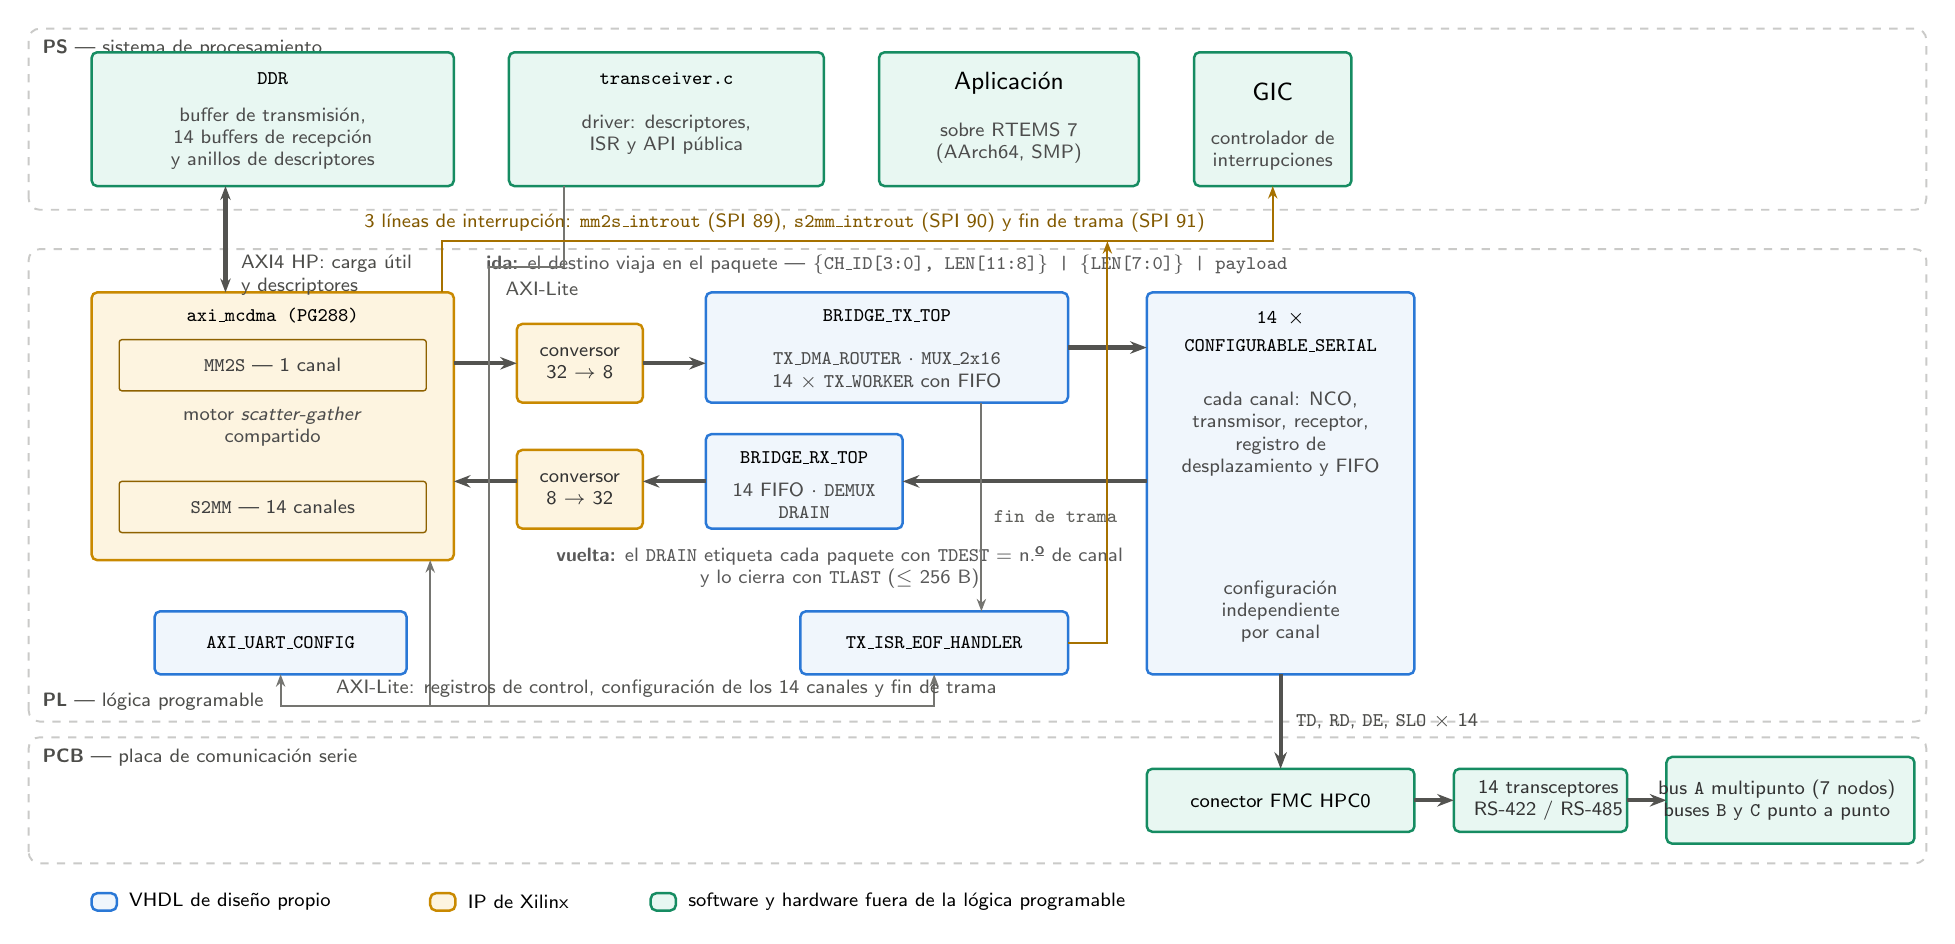
\begin{tikzpicture}[
    x=1cm, y=1cm, font=\sffamily\small,
    blk/.style={draw=cPropio, line width=0.9pt, rounded corners=2pt,
                fill=cPropio!7},
    ip/.style={draw=cIP!85!black, line width=0.9pt, rounded corners=2pt,
               fill=cIP!12},
    ext/.style={draw=cExt!80!black, line width=0.9pt, rounded corners=2pt,
                fill=cExt!10},
    band/.style={draw=cRef!45, dashed, line width=0.7pt, rounded corners=4pt},
    sig/.style={-{Stealth[length=4.5pt]}, line width=0.7pt, cRef!85!black},
    stream/.style={-{Stealth[length=6pt]}, line width=1.5pt, cRef!60!black},
    irq/.style={-{Stealth[length=4.5pt]}, line width=0.7pt, cIP!70!black},
    lbl/.style={font=\sffamily\scriptsize, inner sep=2pt},
    tlbl/.style={font=\ttfamily\scriptsize, inner sep=2pt},
    name/.style={font=\ttfamily\scriptsize, align=center},
    sub/.style={font=\sffamily\scriptsize, align=center, text=black!70},
    note/.style={font=\sffamily\scriptsize, align=center, text=black!65,
                 fill=white, inner sep=2pt},
]

% ===================== Bandas =====================
\draw[band] (-0.2,8.45) rectangle (23.9,10.75);
\node[lbl, anchor=north west, text=cRef!55!black] at (-0.1,10.68)
      {\textbf{PS} --- sistema de procesamiento};

\draw[band] (-0.2,1.95) rectangle (23.9,7.95);
\node[lbl, anchor=south west, text=cRef!55!black] at (-0.1,2.02)
      {\textbf{PL} --- lógica programable};

\draw[band] (-0.2,0.15) rectangle (23.9,1.75);
\node[lbl, anchor=north west, text=cRef!55!black] at (-0.1,1.68)
      {\textbf{PCB} --- placa de comunicación serie};

% ===================== PS =====================
\draw[ext] (0.6,8.75) rectangle (5.20,10.45);
\node[name] at (2.90,10.12) {DDR};
\node[sub] at (2.90,9.35) {buffer de transmisión,\\14 buffers de recepción\\y anillos de descriptores};

\draw[ext] (5.90,8.75) rectangle (9.90,10.45);
\node[name] at (7.90,10.12) {transceiver.c};
\node[sub] at (7.90,9.40) {driver: descriptores,\\ISR y API pública};

\draw[ext] (10.60,8.75) rectangle (13.90,10.45);
\node[align=center] at (12.25,10.05) {Aplicación};
\node[sub] at (12.25,9.30) {sobre RTEMS 7\\(AArch64, SMP)};

\draw[ext] (14.60,8.75) rectangle (16.60,10.45);
\node[align=center] at (15.60,9.95) {GIC};
\node[sub] at (15.60,9.20) {controlador de\\interrupciones};

% ===================== PL: motor de DMA =====================
\draw[ip] (0.60,4.00) rectangle (5.20,7.40);
\node[name] at (2.90,7.10) {axi\_mcdma (PG288)};
\draw[draw=cIP!60!black, line width=0.5pt, rounded corners=1pt]
      (0.95,6.15) rectangle (4.85,6.80);
\node[sub, text=black!75] at (2.90,6.48) {\texttt{MM2S} --- 1 canal};
\node[sub] at (2.90,5.70) {motor \textit{scatter-gather}\\compartido};
\draw[draw=cIP!60!black, line width=0.5pt, rounded corners=1pt]
      (0.95,4.35) rectangle (4.85,5.00);
\node[sub, text=black!75] at (2.90,4.68) {\texttt{S2MM} --- 14 canales};

% ===================== PL: conversores de anchura =====================
\draw[ip] (6.00,6.00) rectangle (7.60,7.00);
\node[sub, text=black!80] at (6.80,6.50) {conversor\\32 $\rightarrow$ 8};
\draw[ip] (6.00,4.40) rectangle (7.60,5.40);
\node[sub, text=black!80] at (6.80,4.90) {conversor\\8 $\rightarrow$ 32};

% ===================== PL: puente de diseño propio =====================
\draw[blk] (8.40,6.00) rectangle (13.00,7.40);
\node[name] at (10.70,7.10) {BRIDGE\_TX\_TOP};
\node[sub] at (10.70,6.40) {\texttt{TX\_DMA\_ROUTER} $\cdot$ \texttt{MUX\_2x16}\\14 $\times$ \texttt{TX\_WORKER} con FIFO};

\draw[blk] (8.40,4.40) rectangle (10.90,5.60);
\node[name] at (9.65,5.30) {BRIDGE\_RX\_TOP};
\node[sub] at (9.65,4.75) {14 FIFO $\cdot$ \texttt{DEMUX}\\\texttt{DRAIN}};

\draw[blk] (9.60,2.55) rectangle (13.00,3.35);
\node[name] at (11.30,2.95) {TX\_ISR\_EOF\_HANDLER};

\draw[blk] (1.40,2.55) rectangle (4.60,3.35);
\node[name] at (3.00,2.95) {AXI\_UART\_CONFIG};

% ===================== PL: transceptores =====================
\draw[blk] (14.00,2.55) rectangle (17.40,7.40);
\node[name, anchor=north] at (15.70,7.28) {14 $\times$};
\node[name, anchor=north] at (15.70,6.92) {CONFIGURABLE\_SERIAL};
\node[sub] at (15.70,5.60) {cada canal: NCO,\\transmisor, receptor,\\registro de\\desplazamiento y FIFO};
\node[sub] at (15.70,3.35) {configuración\\independiente\\por canal};

% ===================== PCB =====================
\draw[ext] (14.00,0.55) rectangle (17.40,1.35);
\node[align=center, font=\sffamily\scriptsize] at (15.70,0.95) {conector FMC HPC0};
\draw[ext] (17.90,0.55) rectangle (20.10,1.35);
\node[sub, text=black!80] at (19.10,0.95) {14 transceptores\\RS-422 / RS-485};
\draw[ext] (20.60,0.40) rectangle (23.75,1.50);
\node[sub, text=black!80] at (22.00,0.95)
      {bus \texttt{A} multipunto (7 nodos)\\buses \texttt{B} y \texttt{C} punto a punto};

% ===================== Camino de datos: transmisión =====================
\draw[stream] (5.20,6.50) -- (6.00,6.50);
\draw[stream] (7.60,6.50) -- (8.40,6.50);
\draw[stream] (13.00,6.70) -- (14.00,6.70);
\node[note, anchor=south] at (10.70,7.55)
      {\textbf{ida:} el destino viaja en el paquete ---
       \texttt{\{CH\_ID[3:0], LEN[11:8]\} | \{LEN[7:0]\} | payload}};

% ===================== Camino de datos: recepción =====================
\draw[stream] (14.00,5.00) -- (10.90,5.00);
\draw[stream] (8.40,5.00) -- (7.60,5.00);
\draw[stream] (6.00,5.00) -- (5.20,5.00);
\node[note, anchor=north] at (10.10,4.24)
      {\textbf{vuelta:} el \texttt{DRAIN} etiqueta cada paquete con
       \texttt{TDEST} = n.\textordmasculine\ de canal\\
       y lo cierra con \texttt{TLAST} ($\leq$ 256~B)};

% ===================== DDR <-> MCDMA =====================
\draw[{Stealth[length=5pt]}-{Stealth[length=5pt]}, line width=1.5pt, cRef!60!black]
      (2.30,8.75) -- (2.30,7.40);
\node[lbl, anchor=west, align=left, text=cRef!55!black] at (2.42,7.62)
      {AXI4 HP: carga útil\\y descriptores};

% ===================== Control: AXI-Lite desde el driver =====================
\draw[sig] (6.60,8.75) -- (6.60,7.72) -- (5.65,7.72) -- (5.65,2.15)
           -- (3.00,2.15) -- (3.00,2.55);
\draw[sig] (5.65,2.15) -- (11.30,2.15) -- (11.30,2.55);
\draw[sig] (4.90,2.15) -- (4.90,4.00);
\node[lbl, anchor=west, text=cRef!60!black] at (5.78,7.45) {AXI-Lite};
\node[lbl, anchor=south, text=cRef!60!black] at (7.90,2.18)
      {AXI-Lite: registros de control, configuración de los 14 canales y fin de trama};

% ===================== Fin de trama: del puente al bloque propio =====================
\draw[sig] (11.90,6.00) -- (11.90,3.35);
\node[tlbl, anchor=west, text=cRef!70!black] at (11.98,4.55) {fin de trama};

% ===================== Interrupciones =====================
\draw[irq] (5.05,7.40) -- (5.05,8.05) -- (15.60,8.05) -- (15.60,8.75);
\draw[irq] (13.00,2.95) -- (13.50,2.95) -- (13.50,8.05);
\node[lbl, anchor=south, text=cIP!55!black] at (9.40,8.09)
      {3 líneas de interrupción: \texttt{mm2s\_introut} (SPI 89),
       \texttt{s2mm\_introut} (SPI 90) y fin de trama (SPI 91)};

% ===================== PL -> PCB =====================
\draw[stream] (15.70,2.55) -- (15.70,1.35);
\node[lbl, anchor=west, text=cRef!55!black] at (15.82,1.95)
      {\texttt{TD}, \texttt{RD}, \texttt{DE}, \texttt{SLO} $\times$ 14};
\draw[stream] (17.40,0.95) -- (17.90,0.95);
\draw[stream] (20.10,0.95) -- (20.60,0.95);

% ===================== Leyenda =====================
\draw[blk] (0.60,-0.45) rectangle (0.92,-0.23);
\node[lbl, anchor=west] at (1.00,-0.34) {VHDL de diseño propio};
\draw[ip] (4.90,-0.45) rectangle (5.22,-0.23);
\node[lbl, anchor=west] at (5.30,-0.34) {IP de Xilinx};
\draw[ext] (7.70,-0.45) rectangle (8.02,-0.23);
\node[lbl, anchor=west] at (8.10,-0.34) {software y hardware fuera de la lógica programable};

\end{tikzpicture}
\end{document}
